\documentclass[conference]{IEEEtran}

\usepackage{amsmath}
\usepackage{algorithm}
\usepackage{algorithmic}
\usepackage{graphicx}
\usepackage{cite}
\usepackage{array}
\usepackage{cases}
\usepackage{booktabs}
\usepackage{multirow}
\usepackage{epsfig}
\usepackage[TABBOTCAP]{subfigure}
\usepackage{esint}

\newtheorem{definition}{Definition}
\newtheorem{theorem}{Theorem}
\newtheorem{proposition}{Proposition}
\newtheorem{corollary}{Corollary}
\newtheorem{lemma}{Lemma}
\newtheorem{remark}{Remark}
\newtheorem{problem}{Problem}
\newcommand{\tabincell}[2]{\begin{tabular}{@{}#1@{}}#2\end{tabular}}


\hyphenation{op-tical net-works semi-conduc-tor}

\hyphenpenalty=5000
\tolerance=1200

\begin{document}

%\title{Alano: May You Discover Your Neighbors in Partially-Connected Networks}
\title{Alano: May You Discover Your Neighbors}

% author names and affiliations
% use a multiple column layout for up to three different
% affiliations

% conference papers do not typically use \thanks and this command
% is locked out in conference mode. If really needed, such as for
% the acknowledgment of grants, issue a \IEEEoverridecommandlockouts
% after \documentclass

% for over three affiliations, or if they all won't fit within the width
% of the page, use this alternative format:
%
%\author{\IEEEauthorblockN{Michael Shell\IEEEauthorrefmark{1},
%Homer Simpson\IEEEauthorrefmark{2},
%James Kirk\IEEEauthorrefmark{3},
%Montgomery Scott\IEEEauthorrefmark{3} and
%Eldon Tyrell\IEEEauthorrefmark{4}}
%\IEEEauthorblockA{\IEEEauthorrefmark{1}School of Electrical and Computer Engineering\\
%Georgia Institute of Technology,
%Atlanta, Georgia 30332--0250\\ Email: see http://www.michaelshell.org/contact.html}
%\IEEEauthorblockA{\IEEEauthorrefmark{2}Twentieth Century Fox, Springfield, USA\\
%Email: homer@thesimpsons.com}
%\IEEEauthorblockA{\IEEEauthorrefmark{3}Starfleet Academy, San Francisco, California 96678-2391\\
%Telephone: (800) 555--1212, Fax: (888) 555--1212}
%\IEEEauthorblockA{\IEEEauthorrefmark{4}Tyrell Inc., 123 Replicant Street, Los Angeles, California 90210--4321}}

\maketitle

\input{abstract}

\IEEEpeerreviewmaketitle

% Introduction
\section{Introduction}

%%%%%%

% Cite:
% Wireless networks			#gupta2000capacity
% Wireless sensor networks	#akyildiz2002wireless
% Volcanic investigation		#werner2006deploying

% Mobile campus networks 	#hernandez2005comparative
% Mobile gaming community	#cunningham2002optimizing
% Energy-efficient network	#jones2001survey
% Internet of things 			#qin2014software
% Connectivity  			#moscibroda2006complexity
% Density					#wang2015connectivity
% Unit disk graph model 		#clark1990unit
% CSMA/CA				#bianchi1996performance

% The cite of the existing algorithms are listed in related work

%%%%%%

% Paper Logic Flow


Wireless sensor networks %~\cite{akyildiz2002wireless} 
are deployed in
a wide range of real-life applications today, such as volcanic investigation~\cite{werner2006deploying}, 
seismic detection~\cite{suzuki2007high},
agriculture monitoring~\cite{wang2010l3sn}, etc.
The popularity of Internet of Things (IoT) will accelerate this trend
and make wireless sensor networks even more pervasive.

In constructing a wireless sensor network,
neighbor discovery is an important fundamental step.
In most situations, a node participating in a task needs to discover its nearest
neighbors in order to carry out operations like broadcasting and peer-to-peer
communication. In this paper, we study neighbor discovery under the
constraint of limited energy. We assume a
large-scale scenario, where nodes are aware of their energy consumption and
are connected via a multi-hop network.

Despite extensive research, neighbor discovery in a large-scale network
%remains an open problem.??
remains a problem that is not fully solved.
Existing algorithms can be classified into two categories: deterministic, and probabilistic.
The algorithms presented in
Refs.~\cite{dutta2008practical, kandhalu2010u, bakht2012searchlight,
sun2014hello, chen2015heterogeneous, qiu2016talk} are %sensors take actions
based on deterministic sequences.
Most deterministic algorithms however were designed for two
nodes only, despite being then applied to a multi-node scenario.
On the other hand,
probabilistic algorithms handle neighbor discovery in a clique of $n$
nodes~\cite{mcglynn2001birthday, vasudevan2009neighbor, you2011aloha,
song2014probabilistic}, i.e. every two nodes are neighbors, and utilize
the global number $n$ to compute an optimal probability for action
decisions. However, a large-scale network is generally not a clique and
node to node communication could go through multiple hops.
In addition, prominent existing
algorithms such as Birthday~\cite{mcglynn2001birthday} and Aloha-like~\cite{vasudevan2009neighbor} 
do not consider energy consumption of the
neighbor discovery process, which could have a negative impact on the
energy state of the sensors.
%Furthermore, in wireless sensor networks,
%sensors are powered by battery and neighbor discovery will be constraint
%to energy limits.

To address the problems identified above, we looked into the existing
neighbor discovery algorithms and found that the key issue lies in the
way collisions are dealt with in large-scale networks.
%(collisions result in CSMA \cite{bianchi1996performance} to wait for more time).
%This issue is due to three reasons.???
There are three aspects to this issue.
First, transmission signals fade with distance and simultaneous
transmissions will cause collisions. %among various nodes.
Deterministic algorithms aiming at two nodes~\cite{kandhalu2010u,
chen2015heterogeneous} fail to reduce such collisions. Some beacon-based
algorithms~\cite{dutta2008practical, bakht2012searchlight, sun2014hello,
qiu2016talk} do not have this problem but their time slot is 40 times
larger~\cite{kandhalu2010u} and therefore resulting in long latency. 
%There are many mature interference models to depict the communication collisions, and we choose the popular protocol model\cite{clark1990unit} to begin this research area.
Second, a large-scale network is not one-hop network and a node can
practically only discover those neighbors that are within its range.
Probabilistic algorithms~\cite{vasudevan2009neighbor, you2011aloha, song2014probabilistic}
assuming a small clique network fail to estimate the number of
neighbors, and thus cannot reduce the collisions effectively since the
number of neighbors provides an important hint on how many collisions
will occur at the same time.
Third, nodes have limited energy and they only have a small time window
to find their neighbors. Indeed, energy conservation and
neighbor discovery are two conflicting goals in existing algorithms.
%since collisions cause great energy consumption and if taken energy consumption into account, neighbor discovery may become even
ineffective.

We have conducted experiments to confirm the issue in real actions.
We deployed $16$ EZ$240$ sensors~\cite{huang2012easipled} and
found existing algorithms to be either insufficient or
excessive in the way they deal with collisions, and
both would result in long latency.
%collisions caused by simultaneous transmissions result in the waste of time and energy. 
%We consider a large-scale network with 2000 nodes obeying a uniform distribution. 
As the number of neighbors increased, collisions of 
Hedis~\cite{chen2015heterogeneous} happened as frequently as 10.1\% to
19.96\%, evoking the CSMA~\cite{bianchi1996performance} function in the MAC
layer to wait for a random time. Hello~\cite{sun2014hello} utilized a
beacon mechanism to avoid collisions but the time slot was 40 times
larger and it resulted in 10 times longer latency. 
An Aloha-like method~\cite{you2011aloha} showed a high idle rate (when no neighbors are
transmitting) of 18.92\%, which reduced the collisions, but
excessively.  %and still results in a high latency.
%This is the same with CSMA \cite{bianchi1996performance}, a general collision avoidance  technique in networks, the idle rate of which is XX\% by simulations. 
All these algorithms could not achieve low latency and energy
conservation at the same time simply because they failed to deal with
collisions effectively.

Our key hypothesis is that, using an estimate of the expected number of
neighbors of a node and synchronizing the times the nodes turn on the
radio, %with its neighbors,
both low-latency and energy-efficiency in neighbor discovery can be achieved. 
We take the distribution of nodes into consideration. As studied
in~\cite{wang2013gaussian}, nodes in a wireless sensor network are
likely to follow a uniform or a Gaussian distribution.
%for detecting aims. % (as shown in Fig. \ref{distribution})
According to the local density, a node can estimate the number of
neighbors and calculate an optimal probability for action decisions.
Based on this, we propose Alano, \footnote{Alano is the god of luck in Greek mythology.}
a nearly optimal probability based algorithm for a large-scale network.
We play on the duty cycle mechanism~\cite{zhang2017performance} 
which is the fraction of time the radio is on
(i.e., the sensor is woken up), and deterministically
synchronize the wake-up times between neighbors in Alano.
Specifically, if all nodes have the same (symmetric) duty cycle, such as
a fleet of sensors having a default duty cycle setting, we propose the
Relaxed Difference Set based algorithm (called RDS-Alano); if nodes have
different (asymmetric) duty cycles, such as when sensors would adjust the duty
cycle according to the remaining energy, we propose the Traversing Pointer based
algorithm (called TP-Alano).

In the simulations, we have found that Alano achieves $31.35\%$ to $ 85.25\%$
lower latency, higher discovery rate, and better scalability in large
scale networks. %, and robustness,
In comparison with the state-of-the-art 
algorithms~\cite{you2011aloha, sun2014hello, chen2015heterogeneous, bakht2012searchlight}
Alano reaches nearly $100\%$ discovery in twice as fast a speed. 
When the number of nodes increases from 1000 to 9000, 
Alano shows 4.68 times to 6.51 times lower latency for neighbor discovery.

% Contribution summarize
The contributions of the paper are summarized as follows:
\begin{itemize}
\item[1)] We utilize the distribution of nodes and propose Alano, a
nearly optimal algorithm that can achieve low-latency neighbor discovery
for a large-scale network.
\item[2)] In an energy-restricted large-scale network, we propose
RDS-Alano for symmetric nodes and TP-Alano for asymmetric nodes. Both
algorithms achieve low latency for discovering neighbors and can prolong
the nodes' lifetime.
\item[3)] We conduct experiments for %fundamental observation
and extensive simulations for large-scale networks, in which
Alano achieves lower latency, higher discovery rate, and better scalability.
The results show Alano's promises for deployment in
%which promises a potential scalability of
IoT in the future.
%, and robustness compared with the state-of-the-art algorithms. 
\end{itemize}

%% Remaining structure
The remainder of the paper is organized as follows. The next section
highlights the related works and their unsolved problems.
Section~\ref{sectionmodel} presents
the system model and basic definitions.
We introduce Alano and show the
method to combine the nodes' distribution in the design
in Section~\ref{PCN}. We propose
two modified algorithms (RDS-Alano, TP-Alano) for an energy-restricted
large-scale network for both symmetric and asymmetric nodes in Section~\ref{EEN}. 
The simulation results are given and discussed in Section~\ref{Evaluation}, 
and we conclude the paper in Section~\ref{Conclusion}.


% Related Work
\section{Related Work}
\label{RW}

%Introduce the representative existing algorithms and their weakness.

%Cite
%Algorithms:

%Deterministic:
%BlindDate 					#wang2015blinddate
%Disco 						#dutta2008practical
%Hello 						#sun2014hello
%Searchlight 					#bakht2012searchlight
%Talk More Listen Less 			#qiu2016talk
%Todis\&Hedis 					#chen2015heterogeneous
%U-Connect  					#kandhalu2010u

%probabilistic:
%Birthday 					#mcglynn2001birthday
%ALOHA-like09 				#vasudevan2009neighbor
%ALOHA-like11 	 			#you2011aloha
%PND 						#song2014probabilistic

%others
%Normal Distribution 			#wang2013gaussian
%Beacon&package 				#mcglynn2001birthday
%RSSI						#daiya2011experimental




Neighbor discovery problem has raised a great deal of attention of scholars \cite{sun2014energy}. 
A number of neighbor discovery methods have been proposed in the past decade.
Technically, these approaches can be classified into two categories, probabilistic and deterministic. 

In the deterministic methods \cite{dutta2008practical,kandhalu2010u,
bakht2012searchlight,sun2014hello,chen2015heterogeneous,
wang2015blinddate,qiu2016talk}, some mathematical techniques, such as
co-primality, quorum system, etc., are utilized to promote the discovery performance.
The deterministic methods holds an obvious advantage that they
can achieve neighbor discovery process within a bounded time latency.

Nevertheless, there exists some crucial weak points in the deterministic algorithm.
Firstly, Disco \cite{dutta2008practical} proposes a discovery protocol that
each node has a capability to send a beacon (one or a few bits) at both beginning and end of
an active slot, which is widely adopted by the later algorithms such as
SearchLight \cite{bakht2012searchlight}, BlindDate \cite{wang2015blinddate}
and Hello \cite{sun2014hello}, Nihao \cite{qiu2016talk}. It is quite an efficient way for two nodes to discover
each other within an ideal time latency. However,  they do not solve the collision 
issues when receiving packages from multiple neighbors. Furthermore, when they are 
extended for multiple nodes, only sending a beacon to discover the neighbors is 
totally insufficient. A node needs to send a complete package 
(some papers still call beacon) containing all its information,
otherwise the neighbor can not  identify which neighbor the beacon belongs to \cite{zhou2004impact}.
Thus a complete time slot is necessary for a node to transmit a package or listen to 
the channel to receive a package.

Another category is probabilistic methods \cite{mcglynn2001birthday,
vasudevan2009neighbor,you2011aloha,song2014probabilistic}. These
approaches utilize probability techniques to promote the randomness 
to discover the neighbors. Different from the deterministic algorithms, 
this kind of method shows an significant strength in the multiple nodes scenario. 
However, probabilistic methods only present an expectation discovery latency and 
can not guarantee a latency bound in the worst case.
In addition, almost all the existing methods consider the network is fully-connected,
the topology of which is a complete graph. Deploying a fully-connected network 
in a large-scale area is technically impractical 
due to the limited sensing range of devices communication.
How far the other node can be detected as a neighbor for a mobile equipment  
depends on criterion such as the received signal strength \cite{daiya2011experimental}.
From our analysis and simulations, 
they show a poor performance in the large-scale networks, where the nodes are
partially-connected.

To the best of our knowledge, neither deterministic nor probabilistic methods are designed for
the networks which are partially-connected. In this paper, we present a low-latency, energy-efficient 
neighbor discovery algorithm for the large-scale networks.

The proposed RDS-Alano and TP-Alano in this paper are a combination of both two categories,
and thus we compare our proposed algorithms with both deterministic and probabilistic methods. 
Particularly as mentioned above, the deterministic approaches need some adjustments 
when transferred to large-scale networks since the protocol can not work. 
Details will be introduced in Section \ref{Evaluation}.






%\section{System Model and Problem Formulation}
\section{Preliminaries}
\label{sectionmodel}

In this section, we first give some notion definitions and introduce the collision detection mechanism. 
Then we formulate the Neighbor Discovery problem formally.  


\subsection{Sensor Node Model}

The wireless sensor network consists of a number of sensors distributed separately in a target area.
The deployed sensor nodes keep their most time in sleep pattern to avoid quick energy consumption 
and wake up timely to work on duty.

In our model, we assume that each node has a unique identifier $ID_i$ which is aware by theirselves, while the total amount of sensors $N$  is not necessary to be known. Time is divided into slots of equal length $t_0$, 
which is sufficient to finish  one communication process(transmit or receive a piece of package). In each time slot, a node transform its pattern according to a pre-defined duty schedule.

\begin{definition}
\textbf{Duty schedule} is a pre-defined sequence $S=\{s^t\}_{0\leq t<T}$ of period $T$ and
$$ s^t=\left\{
\begin{aligned}
0  & & {sleep}\\
1  & & {wake}\\
\end{aligned}
\right.
$$
\end{definition}

 Each node construct its own duty schedule according to a specific strategy and repeats it
 until finding all the neighbors. Since the waking-up duration has a significant affect on the battery's lifetime, 
 duty circle is defined to restrict the energy consumption.

\begin{definition}
\textbf{Duty circle} represents the fraction of one period T where a node turns its radio on. It can be formulated as:

$$\theta=\frac{|\{ 0\leq t<T : s^t =1\}}{T}.
$$
  
\end{definition}

When a sensor wake up on a time slot, it can turn to either the transmitting state or listening state. 
\begin{itemize}
\item \textbf{Transmitting state}. A node turn to transmitting state will broadcast a package containing its own identify 
information to all neighbors.
\item  \textbf{Listening state}. A node turn to listening state will monitor the frequency channel to collect its neighbors' packages.
However collision will occur when two or more neighbor nodes transmit concurrently and thus no valid information will be gathered
\end{itemize}
Transiting between the states only costs little time, compared to one complete time slot.

%@@@
\subsection{Collision Detection Mechanism}

When a node wakes up and turns to the listening state, there are two possible 



A collision detection mechanism allows the node to distinguish these two case, in turn is 


A node turns to listening state when it wakes up
%@@@




\subsection{Problem Definition}

We consider a partially-connected sensor network, 
where two nodes are neighbors if they locate within the radio range of each other. 
A  symmetric matrix $M_{N\times N}$ is used to record the neighboring relations as:

$$ M_{i,j}=\left\{
\begin{aligned}
1  & & & & & & {connected}\\
0  & & & & & & {disconnected}\\
\end{aligned}
\right.
$$

Each sensor follows its duty schedule to achieve neighbor discovery. In a synchronous scenario,
sensors start their neighbor discovery process at the same time, while in a asynchronous  scenario
all nodes start at different time slots.
 
Notice that the neighbor discovery process is not bidirectional, which means any pair of neighbors 
need to find each other separately. The time slots within which a sensor node $u_i$ find one of its neighbors $u_j$ can be formulated 
as $L(i,j)$. Then we define the discovery latency that node $u_i$ discovers all neighbors as:

\begin{definition}
\textbf{Discovery latency} of node $u_i$ is the time to discover all neighbors:
$$L(i) = \max_{M_{i,j = 1}} L (i,j).
$$
\end{definition}

Thus the neighbor discovery problem can be formulated as:
%@@@
\begin{problem}
Given a duty circle $\theta$, design a duty schedule and transiting strategy which optimizes $L(i)$ to the most extent. 
\end{problem}
%@@@





\section{Partially-Connected Networks}
\label{PCN}



%background and instances
A practical scenario is that in a network,
all the nodes are partially connected with each other
In a partially-connected network, the nodes 
within their 


%density function and expectation of the neighbor number
In a partially-connected network for $\forall$ node $u_i$, 
its position coordinate $(x_i,y_i)$
obeys a certain probability distribution depending on the 
characteristic of the network, with the density function as :
$$f(x,y)=
\begin{cases}
\varphi(x,y)& (x,y)\in D\\
0& (x,y)\notin D
\end{cases}$$
where $D$ is the network covering area.

$\forall$ node $u_i (x_i,y_i)$, its sensing range area $R_i$ can be formulated as:
$$
(x-x_i)^2+(y-y_i)^2 \leq r^2
$$
where $r$ is the the furthest detection distance.

Thus, we can obtain the neighbor expectation number of node $u_i$ as :
$$
NB(u_i) = N\iint_{R_i} f(x,y)\,dx\,dy - 1.
$$

We ignore the boundary area of the network and assume the
nodes in the network is of an enormous quantity, thus the 
expectation neighbors can be formulated as:
$$
NB(u_i) = N\iint_{R_i} \varphi(x,y)\,dx\,dy.
$$

Note that, when the network area is far more larger than the
sensing area of the nodes, we can approximately get:
$$
NB(u_i) = N\pi r^2 \varphi(x,y).
$$




%Alano
Then we propose \textbf{Alano}, a randomized neighbor discovery algorithm. 
We describe the algorithm for $\forall$ node $u_i$ as Alg. \ref{Alano}.
Alano algorithm indicates that what probability for a node choose to turn to  
tramisitting state or listening state is determined
by the expectation neighbor number varying from node to node.


\begin{algorithm}
\caption{Alano Algorithm}
\label{Alano}
\begin{algorithmic}[1]
\STATE $\hat{n_i} = N\iint_{R_i} \varphi(x,y)\,dx\,dy$;
\STATE $p_t^i = \frac{1}{\hat{n_i}}$;
\WHILE {$True$}
	\STATE A random float $\epsilon \in (0,1)$;
   	 \IF{$\epsilon < p_t$}
    		\STATE Transmit a message containing node information of $u_i$;
	\ELSE
    		\STATE Listen on the channel and decode the node information if receive a message successfully;
	\ENDIF
\ENDWHILE
\end{algorithmic}
\end{algorithm}

In the following section \ref{uniform}, we first consider a general situation that the nodes
in the network are uniform distributed. We derive a proof that the probability
chosen in Alano is the optimal one and show the bounded latency will not 
be much larger than its expectation. Then in the section  \ref{normal} we describe a more
common situation that the nodes in the network obey normal distribution, we present a 
approximately analysis that the discovery latency will not be much larger than uniform distribution.


\subsection{Uniform Distribution}
\label{uniform}
%background
There are a part of partially-connected networks obeying uniform distribution. 
For instance, consider there is a  wireless sensor network carrying out a task of
measuring temperature and humidity in a target area. 
Thus the sensors are supposed to be evenly deployed and the density function can be 
formulated as:
$$f(x)=
\begin{cases}
\frac{1}{A}& (x,y)\in D\\
0& (x,y)\notin D
\end{cases}$$
where $A$ is the dimension of $D$.

Every node in the network has the same expectation 
of neighbor number and thus transmit with the same probability as:
$$
\hat{n} = \frac{N\pi r^2}{A}, \quad p_t = \frac{1}{\hat{n}}=\frac{A}{N\pi r^2}.
$$  

According to Alano, the probability that node $u_i$ discover a specific
neighbor successfully in a time slot is:
$$
p_s = p_t{(1-p_t)}^{\hat{n}-1}.
$$
Let:
$$
p_s' = {(1-p_t)}^{\hat{n}-1}-(\hat{n}-1)p_t{(1-p_t)}^{\hat{n}-2}=0.
$$
It is easy to confirm that  when
$$p_t=\frac{1}{\hat{n}}.$$ 
$p_s$ gets maximum value:
$$p_s = \frac{1}{\hat{n}}{(1-\frac{1}{\hat{n}})}^{\hat{n}-1} \approx \frac{1}{\hat{n}e}.$$

Thus we can conclude that the probability chosen in Alano
to transmit is the optimal one. 

Next we analyse the expectation latency for a node to discover all its 
neighbors. We denote $W_j$ to be a random variable that a new neighbor
is discovered after the node has discovered $(j-1)$ neighbors, which follows 
Geometric distribution with parameter $p(j): p(j)=(\hat{n}-j+1)p_s$. Then the expectation
of $W_j$ is computed as:
$$
E[W_j]=\frac{1}{p(j)}=\frac{1}{(\hat{n}-j+1)p_t}
$$

The expectation time latency of discovering all the neighbors can be formulated as:
$$
E(W_j) = \sum_{j=1}^{\hat{n}}\frac{1}{p_s}H_n \approx ne(lnn + O(1)) = O(nlnn).
$$
where $H_n$ is the $n$-th Harmonic number, i.e.,
$H_n = lnn + O(1)$.

We get the expectation discovery lantecy is within O(nlogn) and then we
show the bounded latency will not be much larger than its expectation.

%To be modified later
%%
For $i\neq j$, $W_i$ and $W_j$ are independent by definition. As $Var[W_j]=\frac{1-p_{suc}(j)}{p^2_{suc}(j)}$ for Geometric distribution with parameter $p_{suc}(j)$, we obtain:

\begin{displaymath}
Var[W]=\sum_{j=1}^{n}Var[W_j]=\sum_{j=1}^{n}\frac{1}{p^2_{suc}(j)}-\sum_{j=1}^{n}\frac{1}{p_{suc}(j)}.
\end{displaymath}
We know that
\begin{displaymath}
\begin{split}
\sum_{j=1}^{n}\frac{1}{p^2_{suc}(j)}%\leq\frac{e^2}{\theta^2}\sum_{j=1}^{p_nN}(\frac{p_nN+\alpha(j-1)}{p_nN-j+1})^2 \\
 %& =\frac{e^2}{\theta^2}\sum_{j=1}^{p_nN}[\alpha^2-\frac{2\alpha p_nN+2\alpha^2p_nN}{j}+\frac{(1+\alpha)^2(p_nN)^2}{j^2}] \\
 \leq\frac{e^2}{\theta^2}[ \alpha^2n-2\alpha n(1+\alpha)H_n
+\frac{\pi^2}{6}(1+\alpha^2)n^2].
\end{split}
\end{displaymath}

According to \emph{Chebyshev¡¦s inequality}, the probability that the discovery time is $2$ times larger than the expectation is:

\begin{displaymath}
\begin{split}
 P[W\ge2E[W]]%=P[|W-E[W]|\ge E[W]]\le\frac{Var[W]}{E[W]^2} \\
%& \le\frac{\sum_{j=1}^{p_nN}\frac{1}{p^2_{suc}(j)}}{(\sum_{j=1}^{p_nN}\frac{1}{p_{suc}(j)})^2}-\frac{1}{\sum_{j=1}^{p_nN}\frac{1}{p_{suc}(j)}} \\
 \leq\frac{e^2\pi^2(1+\alpha^2)/6}{[(1+\alpha)H_n-\alpha]^2}-\frac{\theta/(en)}{[(\alpha+1)H_n-\alpha]}.
\end{split}
\end{displaymath}

It is close to $0$ when $n$ is large. Hence, the latency is not likely to be $2$ times larger than the expectation. Therefore,
\begin{equation}
W=O(nlnn).
\end{equation}

In a word, Alano-NCD and Alano-WCD both are bounded by $O(nlnn)$.

%%



%*****************



The expectation neighbor number of each node:





\subsection{Normal Distribution}
\label{normal}

For , denote the neighbors of 

$$
p_{suc} = (1-p_t^i)p_t^{ij}\prod_{ k=1}^{\hat{n_i}, k\neq j}(1-p_t^{ik})
$$







%\section{Energy-Efficient Networks}
%\section{Modified Alano Algorithms for Energy-Restricted Networks}
\section{Modified Alano for An Energy-Restricted Network}
\label{EEN}
%wireless sensor networks: duty cycle
In an energy-restricted network, nodes have limited energy and designing duty schedule for a node needs to take its duty cycle into account. Obviously, a lower duty cycle implies a larger discovery latency since the node turns its radio off for more time during the schedule. 

In the preceding section, energy constraint is not a crucial factor in Alano; and we design Alano for both symmetric nodes and asymmetric nodes.
%an overview of the motivation of the algorithm
Our initiative idea is to synchronize the slots that the radio is on with the neighbors in a bounded time; then invoke Alano algorithm to achieve low-latency neighbor discovery. 


\subsection{RDS-Alano for Symmetric Nodes}


%Consider Global Duty Circle
Symmetric nodes have the same duty cycle $\theta_i = \theta_j = \theta$, $\forall u_i, u_j$. We utilize Relax Difference Set (RDS) to synchronize time slots that nodes are in transmitting or listening state.


%Introduction of RDS and the property
%*High coincidence of another existing paper && to be altered later
RDS is an efficient tool to construct cyclic quorum systems\cite{jiang2005quorum,luk1997two}. The definition is:
\begin{definition}
A set $R=\{a_1,a_2,...,a_k\} \subseteq Z_n$ (the set of all non-negative integers less than $n$)
is called a RDS if for every $d \neq 0$ (mod $n$),
there exists at least one ordered pair $(a_i,a_j)$ such that $a_i - a_j \equiv d$ (mod $n$), where $a_i,a_j \in D$.
\end{definition}


It has been proved that any RDS must have cardinality $|R| \geq \sqrt{N}$\cite{luk1997two}.
We present a linear algorithm to construct a RDS with cardinality $\lceil \frac{3\sqrt{N}}{2}  \rceil$ under $Z_N$ in Alg. \ref{RDS}.
%*High coincidence


%RDS construction
\begin{algorithm}[!h]
\caption{RDS construction under $Z_N$}
\label{RDS}
\begin{algorithmic}[1]
\STATE $R :=\emptyset$; $\lambda :=\lceil \sqrt{N}  \rceil$,$\mu :=\lceil \frac{\lceil \sqrt{N} \rceil}{2} \rceil$;\label{RDSline1}
\FOR{$i = 1 :\lambda$}
	\STATE $R :=R \cup i$; \label{RDSline2}
\ENDFOR
\FOR{$j = 1 :\mu$}
	\STATE $R :=R \cup (1 + j * \lambda )$; \label{RDSline3}
\ENDFOR
\end{algorithmic}
\end{algorithm}


The intuitive idea of Alg. \ref{RDS} can be described as Fig. \ref{matrix}.
The framed elements are selected as Line. \ref{RDSline2} and Line. \ref{RDSline3}.
We show the correctness of the construction formally.

\begin{figure}[!h]
\centering
\includegraphics[width=2in]{./Figure/matrix}
\caption{An Sketch of RDS construction in Alg. \ref{RDS}}
\label{matrix}
\end{figure}


%The correctness proof of the construction
\begin{lemma}
\label{RDS1}
Set $R = \{r_0, r_1, ..., r_{\lambda + \mu - 1}\}$ constructed in Alg. \ref{RDS} is a RDS,
where $|R| = \lambda + \mu = \lceil \sqrt{N}  \rceil + \lceil \frac{\lceil \sqrt{N} \rceil}{2} \rceil
\approx \lceil \frac{3\sqrt{N}}{2}  \rceil$.
\end{lemma}


\begin{IEEEproof}
Obviously, if there exists one ordered pair $(a_i,a_j)$ satisfying  $a_i - a_j \equiv d$ (mod $N$),
an opposing pair $(a_j,a_i)$ exists such that
$a_j - a_i \equiv (N-d)$ (mod $N$). Thus we only need to find
at least one ordered pair $(a_i,a_j)$ for each $d \in [1, \lfloor N/2 \rfloor]$.

In the construction, $\lambda$ in Line \ref{RDSline1} is the smallest integer satisfying
$\lambda^2 \geq N$. Every $d$ within range $[1, \lfloor N/2 \rfloor]$
can be represented as: $ d = 1 + j \times \lambda - i$, where $1 \leq j \leq \mu,
1 \leq i \leq \lambda$. Thus, there exists $a_j = 1 + j \times \lambda$
from Line. \ref{RDSline2} and $a_i = i$ from Line. \ref{RDSline3}
satisfying  $a_j - a_i \equiv d$. Then, the lemma can be derived.
\end{IEEEproof}


%RDS Based Alano Algorithm
For symmetric nodes with duty cycle $\theta$, we present a RDS based Alano (RDS-Alano) algorithm as Alg. \ref{RDS-ND}.

In Alg. \ref{RDS-ND}, RDS is used to construct a deterministic
schedule for a node to turn on its radio in every period of length $T$,
and Alano is utilized as a probabilistic strategy to
determine whether it is in transmitting state or listening state.

\begin{algorithm}
\caption{RDS Based Alano Algorithm}
\label{RDS-ND}
\begin{algorithmic}[1]
\STATE $T := \lceil \frac{9}{4\theta^{2}} \rceil$; $t := 0$;
\STATE Invoke Alg. \ref{RDS} to construct the RDS $R = {r_0, r_1, ...,r_{\lceil \frac{3\sqrt{T}}{2}  \rceil}}$ under $Z_T$;
\WHILE {$True$}
   	 \IF{$(t + 1) \in R$}
    		\STATE Invoke Alg. \ref{Alano} to determine transmission state;
	\ELSE
    		\STATE Sleep;
	\ENDIF
	\STATE t := (t + 1) \% T;
\ENDWHILE
\end{algorithmic}
\end{algorithm}

%The time bound analysis   dutycycle zhengming

We derive discovery latency bound for RDS-Alano:

\begin{theorem}
\label{theoremRDS}
RDS-Alano guarantees that the discovery latency of a node
is bounded within $O(\frac{n\log n}{\theta^2})$ with high probability.
\end{theorem}

\begin{IEEEproof}
First, we verity that the duty cycle in RDS-Alano (denote as $\widetilde{\theta}$) is
$$
\widetilde{\theta} = \frac{|RDS|}{|T|} = \frac{\lceil \frac{3\sqrt{T}}{2}  \rceil}{T} = \theta.
$$

For any pair of neighbor nodes ($u_i$, $u_j$),
we can find an ordered pair ($r_i$, $r_j$) from their respective RDS
such that $r_i - r_j \equiv \delta_{ij}$ (mode $T$), where $\delta_{ij}$ is the time drift.
This implies any neighbor nodes can turn on their radios in the same time slot for at least once during every period of length $T$. 
Regarding each period of $T$ time slots as a `super' slot of Alano algorithm, we can derive that the discovery latency is bounded within $O(\frac{n\ln n}{\theta^2})$ slots with high probability by combining the analysis of Alano.
\end{IEEEproof}

\begin{remark}
In a RDS, a node can discovery its neighbors in different time slots. When treating a period of $T$ as a  `super' slot of Alano, 
there may be less than the total neighbors in each wake-up sub-slot,
resulting less collisions and lower latency compared to when all the neighbors wake up in the same sub-slot.
Thus the latency bound can not be larger.
\end{remark}


\subsection{TP-Alano for Asymmetric Nodes}


%Consider Local Duty Circle
Considering a more practical network where nodes can adjust their duty cycles, we present a traversing pointer method to synchronize time slots that nodes are in transmitting or listening state for asymmetric nodes.


For a more practical scenario, the nodes in a wireless sensor networks may be assigned to diverse tasks such as weather monitoring,
temperature measurement, etc., and thus ought to have asymmetric capability of
battery-management with local duty cycle $\theta_i$.

Suppose the duty cycle of node $u_i$ is $\theta_i$, we present a traversing pointer based Alano (TP-Alano) algorithm as Alg. \ref{P-ND}.
In each period of $T$ slots, a node turns on its radio in two different time slots, one of which is the
first slot of each period and the other one is a traversing slot that changes from period to period (as described in Line. \ref{P-NDline1}).

%Prime Based Neighbor Discovery Algorithm
\begin{algorithm}[!h]
\caption{Traversing Pointer Based Alano Algorithm}
\label{P-ND}
\begin{algorithmic}[1]
\STATE $T :=$ the smallest prime no less than $\frac{2}{\theta_i}$; $t := 0$;
\WHILE {$True$}
	\STATE $t_1 := t \% T$;
	\STATE $t_2 : =\lfloor t / T \rfloor \% (T - 1) +1$;\label{P-NDline1}
   	 \IF{$t_1 = 0~or~t_1 = t_2$}
    		\STATE Invoke Alg. \ref{Alano} to determine transmission state;
	\ELSE
    		\STATE Sleep;
	\ENDIF
	\STATE $t := t + 1$;
\ENDWHILE
\end{algorithmic}
\end{algorithm}

We call the first time slot of each period as \emph{fixed pointer} and the traversing
slot as \emph{traversing point}. The pointers are designed to guarantee that nodes $u_i, u_j$
could turn on their radio simultaneously in very period of length $T_i T_j$. A sketch of the pointers is described in Fig. \ref{TP}.

Note that, a period of $T$ slots is constructed as Line 1 where we try to \emph{find the smallest prime $\geq \frac{2}{\theta_i}$},
then it is likely to make the duty cycle of each period smaller than the expected one. This can be easily solved by selecting random slots to turn on the radio for listening in each period $T$, to conform to the expected duty cycle.


\begin{figure}[!h]
\centering
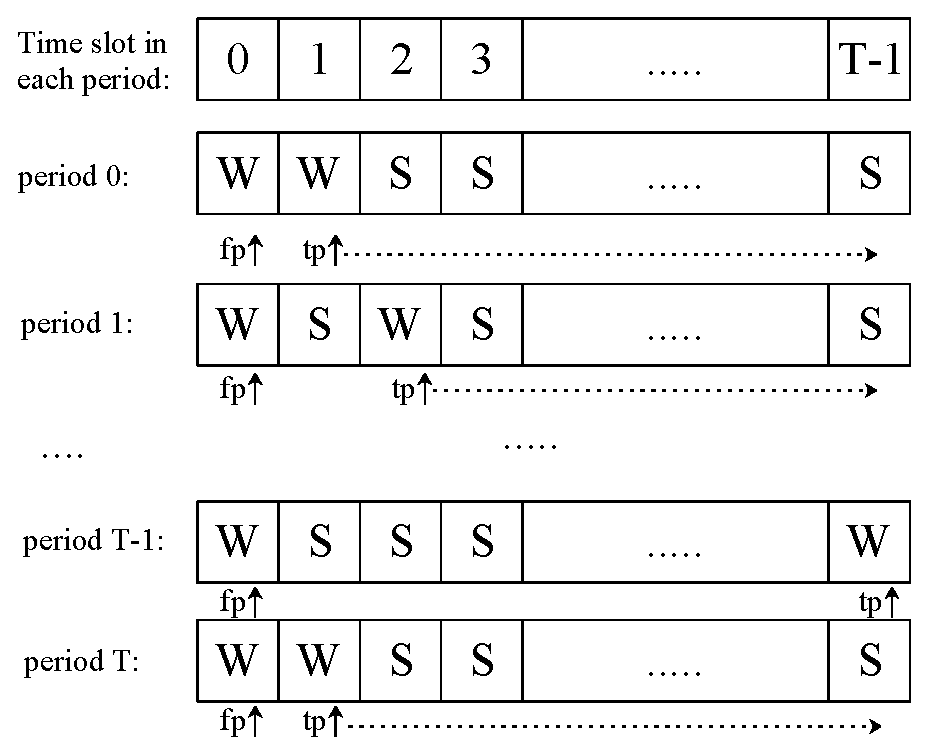
\includegraphics[width=2in]{./Figure/TP}
\caption{A sketch of TP construction in Alg. \ref{P-ND}}
\label{TP}
\end{figure}

%The correctness proof of the construction and the time bound analysis
We show the discovery latency of TP-Alano algorithm as:


\begin{theorem}
\label{PBND1}
TP-Alano guarantees that the discovery latency $L(i,j)$
is bounded within $O(\frac{nlogn}{\theta_i\theta_j})$ with high probability.,
where $\theta_i$ and $\theta_j$ are the duty cycles of
a pair of neighbors ($u_i$, $u_j$) respectively.
\end{theorem}



\begin{IEEEproof}
We first prove that any pair of nodes ($u_i$, $u_j$) turn on their radios (for transmitting or listening) simultaneously for at least once in every period of length $T_iT_j$.

\textbf{Case 1: $T_i \neq T_j$}. Since $T_i$ and $T_j$ are different primes,
according to Chinese Remainder Theorem\cite{ding1996chinese}, there exists a time slot $t_\tau \in \lbrack 0,T_iT_j ) $ satisfying:
\begin{equation}
\label{case1.1}
0 = t_\tau  \quad mod \quad  T_i.
\end{equation}
\begin{equation}
\label{case1.2}
\delta_{ij} = t_\tau  \quad mod \quad  T_j.
\end{equation}

Thus, there exists a fixed pointer of node $u_i$
and a fixed pointer of node $u_j$ in which both nodes turn on the radios in every period of length $T_iT_j$  .

\textbf{Case 2: $T_i = T_j$}. Since $T_i = T_j = T$, if the time drift between $u_i$ and $u_j$ is $\delta_{ij} = 0$, the fixed pointers of $u_i$ and $u_j$ will be the same in every period of length $T$.
Otherwise, since the traversing point will traverse all the time slots once during period of length $(T-1)T$,
there exists a traversing point of $u_i$ and a fixed pointer
of $u_j$ satisfying that both nodes turn on the radios simultaneously in every period of length $(T-1)T$; similarly a traversing point of $u_j$ and a fixed pointer of $i$ satisfying that they both turn on the radios.

Thus for any pair of neighbor nodes ($u_i$, $u_j$), they turn on their radios for transmitting or listening for at least once in every period of length $T_iT_j$. Considering
the whole period $T_iT_j$ to be a 'super' slot of Alano, we derive that the discovery latency is bounded within $O(\frac{n\ln n}{\theta_i\theta_j})$ with high probability.
\end{IEEEproof}








% Evaluation
\section{Evaluation}
\label{Evaluation}


We implemented Alano in C++ and evaluated the algorithms in a cluster of 9 servers, 
each equipped with an Intel Xeon 2.6GHz CPU with 24 hyper-threading cores, 64GB memory and 1T SSD. 

We simulated the network that follows uniform distribution and normal distribution respectively. 
We consider 500 nodes with radio range 10 in $100\times100$ area following uniform distribution, 
and more generally, 1000 nodes with radio range 5 following normal distribution $N(50, 15^2)$. 
The duty cycle is $0.1$, and each time slot represents $20ms$. 
These settings make the network more complicated and realistic than that in 
\cite{wang2015blinddate, qiu2016talk, sun2014hello, bakht2012searchlight, 
chen2015heterogeneous, kandhalu2010u, you2011aloha, 
mcglynn2001birthday, song2014probabilistic, vasudevan2009neighbor}.



We evaluated discovery latency of Alano, Aloha-like~\cite{you2011aloha}, Hello~\cite{sun2014hello}, Hedis~\cite{chen2015heterogeneous}, and Searchlight~\cite{bakht2012searchlight} in partially-connected network. As the deterministic algorithms, Hello, Hedis and Searchlight, only have two states, $\{ON, OFF\}$, we generally assume that when nodes are in $\{ON\}$ state, they transmit and listen with equal probability.
We show that Alano has lower latency, higher discovery rate, and better scalability.

\subsection{Speed: Discovery Latency}

\begin{figure}[!h]
\centering
\subfigure[Uniform Distribution]{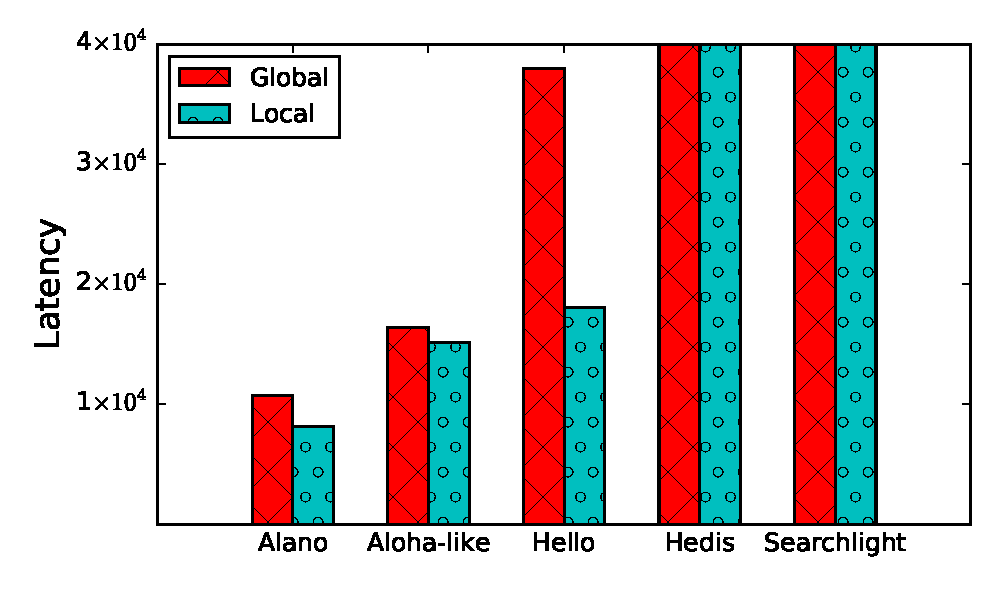
\includegraphics[width=1.65in]{Figure/latency_uniform}}
\hspace{0.01in}
\subfigure[Normal Distribution]{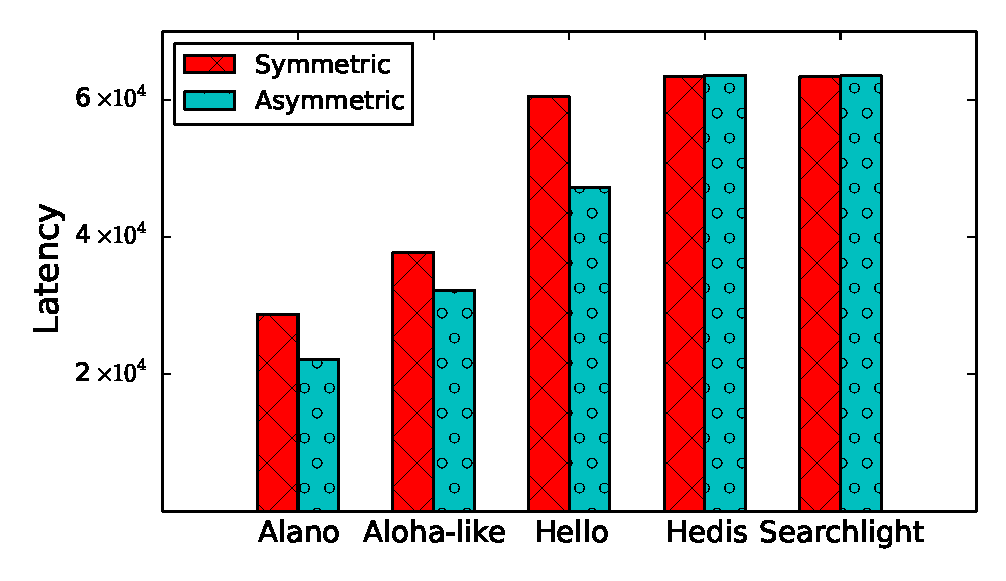
\includegraphics[width=1.65in]{Figure/latency_normal}}
\caption{Alano achieves lower latency.}
\label{fig_latency}
\end{figure}

In Fig. \ref{fig_latency}, when nodes follow uniform distribution, Alano has $53.67\%$ to $5.33$ times lower latency with gloabal duty cycle, and $86.49\%$ to $7.43$ times lower latency with local duty cycle. 
When nodes follow normal distribution, Alano has $31.35\%$ to 24.57 times lower latency with gloabal duty cycle, and $45.94\%$ to $32.32$ times lower latency with local duty cycle. 
The deterministic algorithms Hello, Hedis and Searchlight have high latency, because their design just considered the bounded latency within two nodes. When the network becomes denser and some nodes have more than one neighbors, they cannot discover rapidly, because collisions happen so frequently.


\subsection{Quality: Discovery Rate}

\begin{figure}[!h]

\subfigure[Uniform Distribution with Global Duty Cycle]{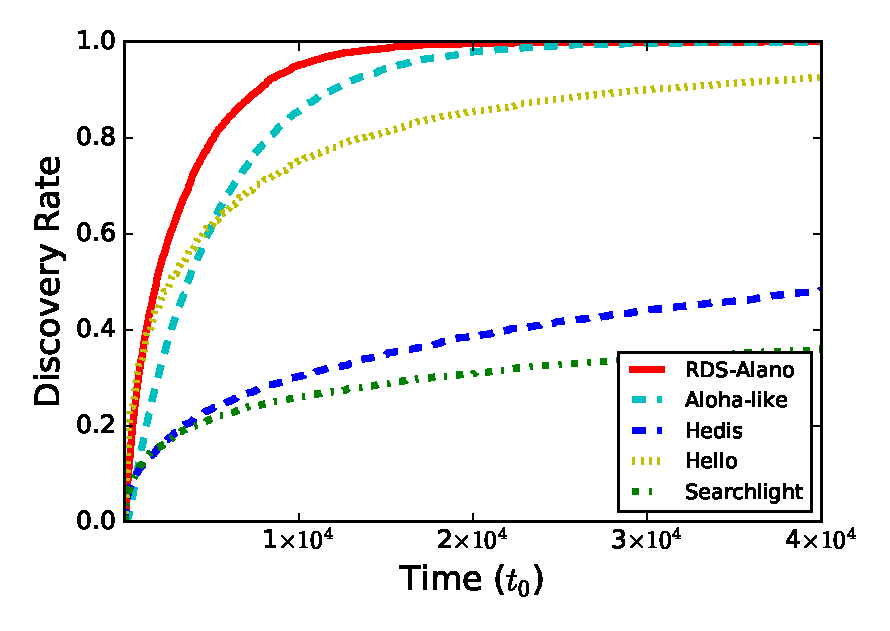
\includegraphics[width=1.65in]{Figure/rate_uniform}}
\hspace{0.01in}
\subfigure[Normal Distribution with Global Duty Cycle]{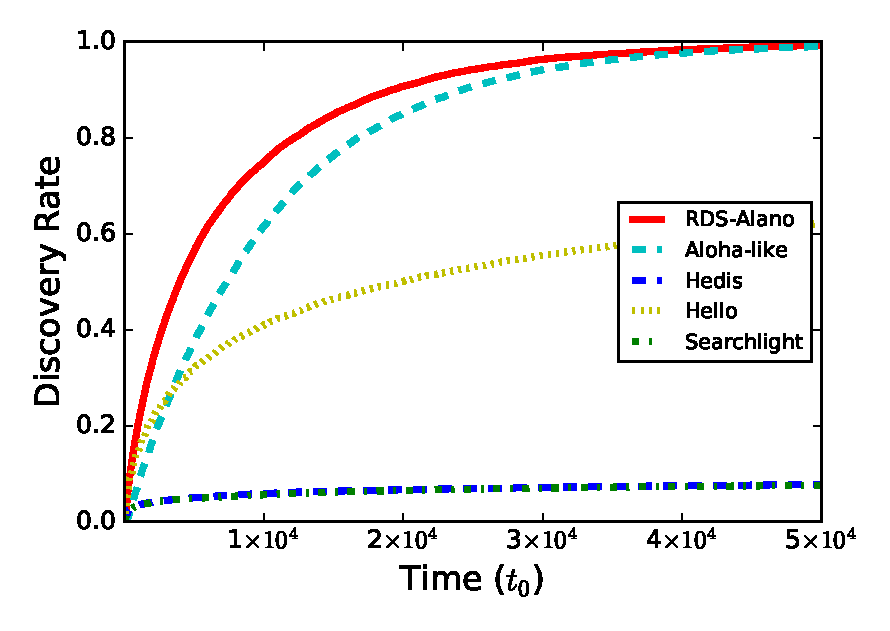
\includegraphics[width=1.65in]{Figure/rate_normal}}
\hspace{0.01in}
\subfigure[Uniform Distribution with Local Duty Cycle]{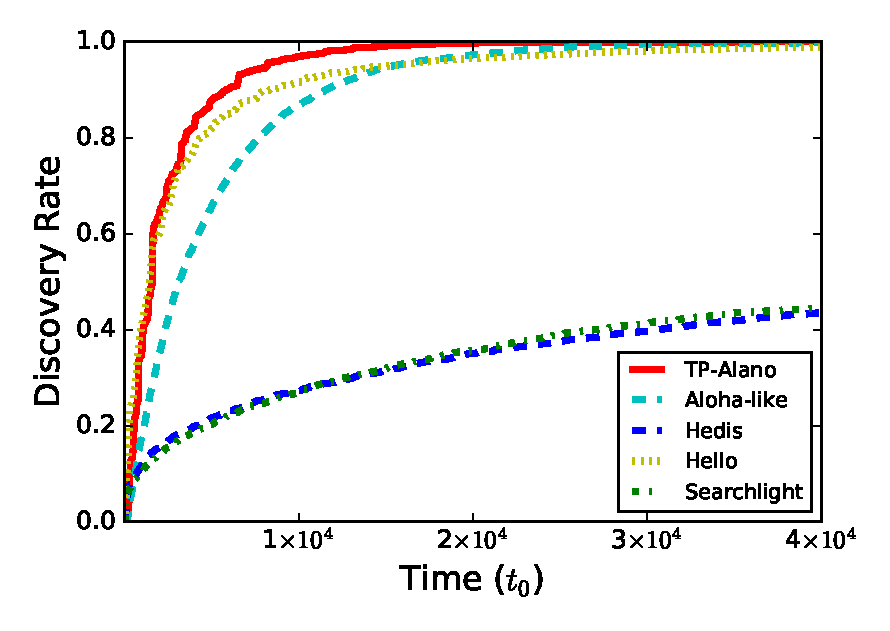
\includegraphics[width=1.65in]{Figure/rate_local_uniform}}
\hspace{0.01in}
\subfigure[Normal Distribution with Local Duty Cycle]{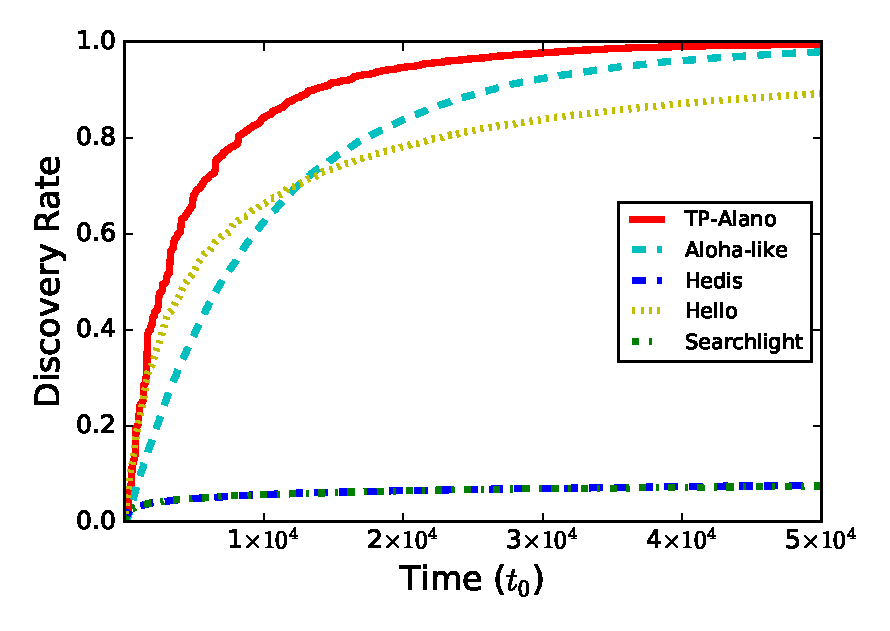
\includegraphics[width=1.65in]{Figure/rate_local_normal}}
\caption{Alano achieves higher discovery rate.}
\label{fig_timerate}
\end{figure}


Fig. \ref{fig_timerate} shows Alano with either global or local duty cycle, has higher discovery rate during the whole course of neighbor discovery in both uniform and normal distribution. The deterministic algorithms Hello, Hedis and Searchlight cannot discover all channels, because of the occurence of collisions. Aloha-like discovers more slowly than Alano when it has discovered a certain number of channels, such as $80\%$ channels in Uniform Distribution with Global Duty Cycle, because it is difficult for pure probabilistic algorithm to deal with the small amount of   undiscovered neighbors.




When we increase the number of nodes in the uniform distributed  network from $500$ to $1000$, and the number of nodes in the normal distributed network from $1000$ to $2000$, Fig. \ref{fig_timerate_large} shows that Alano still reaches higher discovery rate all the time with either global or local duty cycle.

\begin{figure}[!h]

\subfigure[Uniform Distribution with Global Duty Cycle]{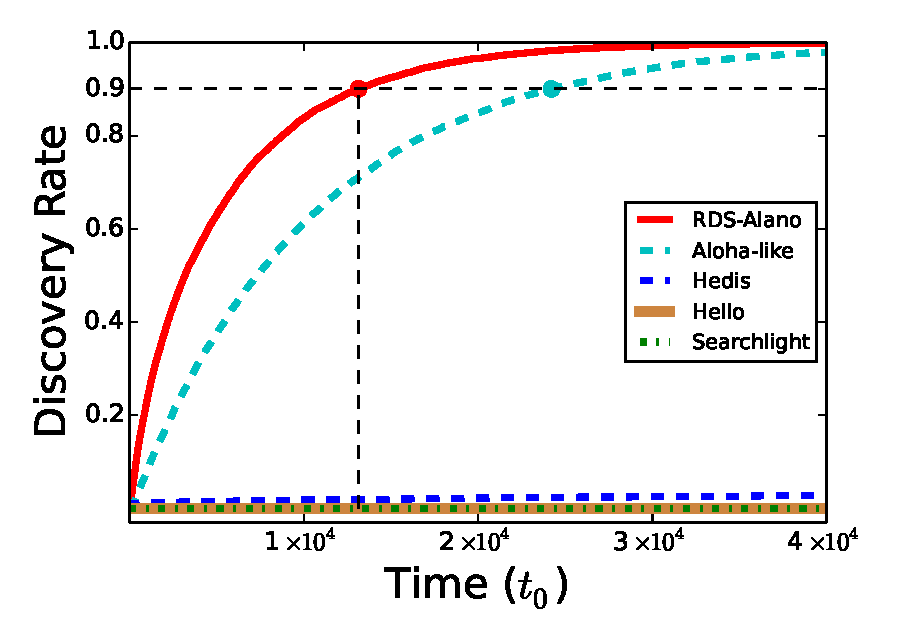
\includegraphics[width=1.65in]{Figure/rate_uniform1}}
\hspace{0.01in}
\subfigure[Normal Distribution with Global Duty Cycle]{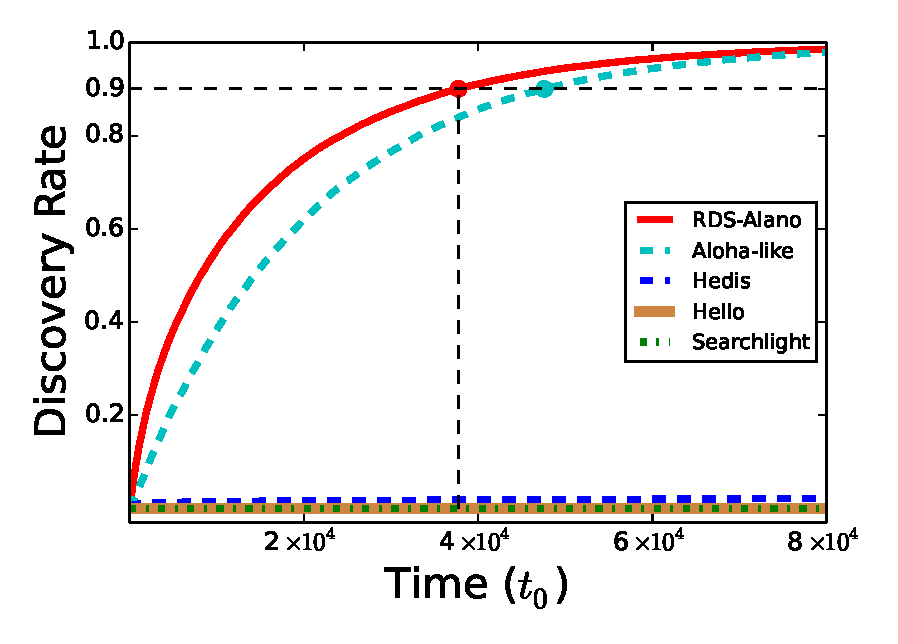
\includegraphics[width=1.65in]{Figure/rate_normal1}}
\hspace{0.01in}
\subfigure[Uniform Distribution with Local Duty Cycle]{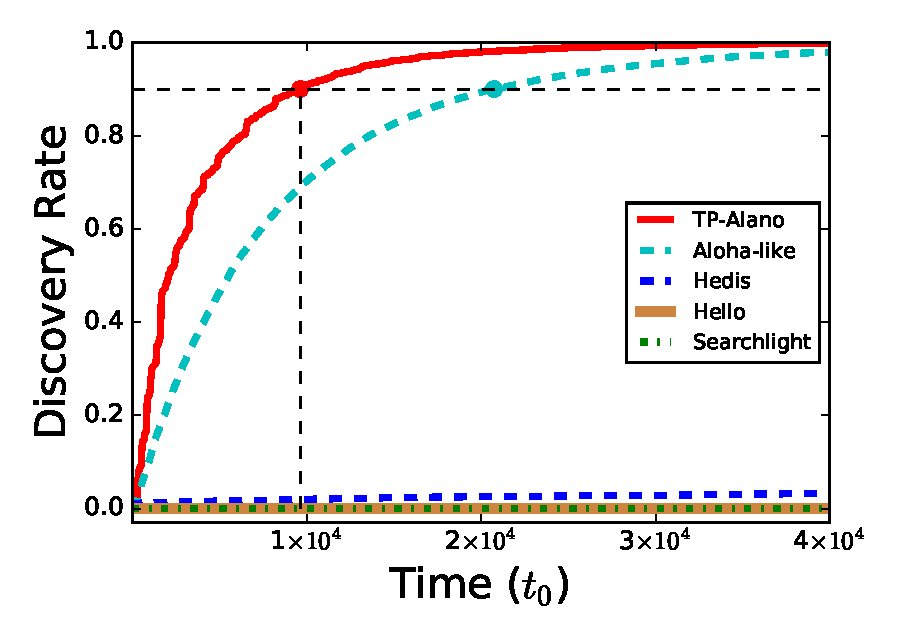
\includegraphics[width=1.65in]{Figure/rate_local_uniform1}}
\hspace{0.01in}
\subfigure[Normal Distribution with Local Duty Cycle]{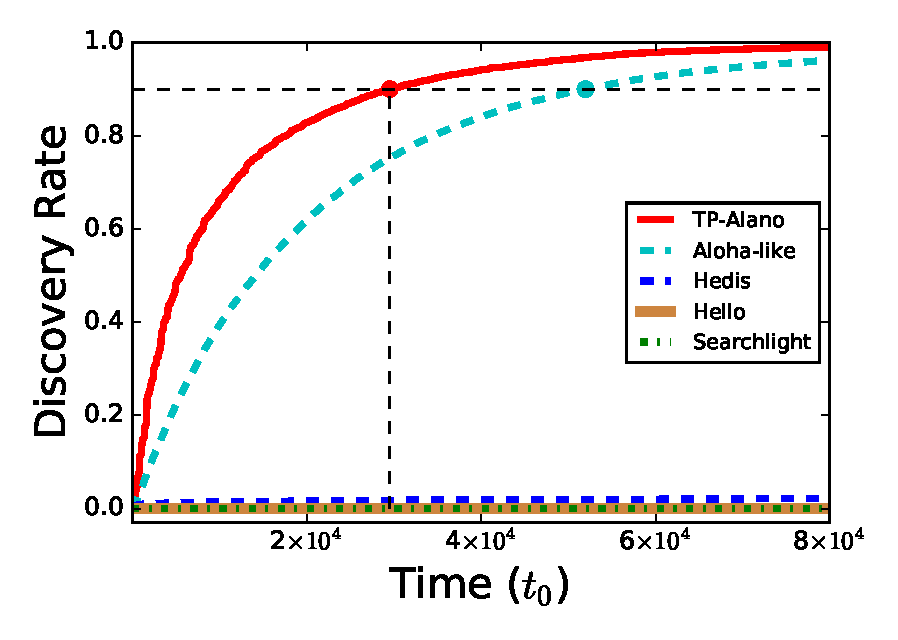
\includegraphics[width=1.65in]{Figure/rate_local_normal1}}
\caption{Alano achieves higher discovery rate in larger networks.}
\label{fig_timerate_large}
\end{figure}





With different duty cycle, Fig. \ref{fig_dutycycle} shows that Alano has lower latency. Compared with Aloha, Alano has from $53.66\%$ to $11.23$ times lower latency. The latency of Alano and Aloha generally decreases as the duty cycle increases, while Hello, Hedis and Searchlight have high latency due to the collision. In normal distribution, Alano has a small twist with duty cycle $0.35$, because when the duty cycle increases, nodes are more likely to transmit and therefore collide.

\subsection{Scalability: Duty Cycle and Network Density}

\begin{figure}[!h]
\centering
\subfigure[Uniform Distribution]{\includegraphics[width=1.65in]{Figure/dutycycle_uniform}}
\hspace{0.01in}
\subfigure[Normal Distribution]{\includegraphics[width=1.65in]{Figure/dutycycle_normal}}
\caption{Alano achieves lower latency in different duty cycle.}
\label{fig_dutycycle}
\end{figure}

\emph{Duty Cycle} 




When the number of nodes increases and the network becomes denser, Alano still shows $50.16\%$ to $4.52$ times lower latency than Aloha-like in uniform distribution and up to $47.03\%$ in normal distribution in Fig. \ref{fig_node}. Here we compare Alano with Aloha-like, because Hello, Hedis and Searchlight can hardly discover neighbors in denser networks. 

\begin{figure}[!h]
\centering
\subfigure[Uniform Distribution]{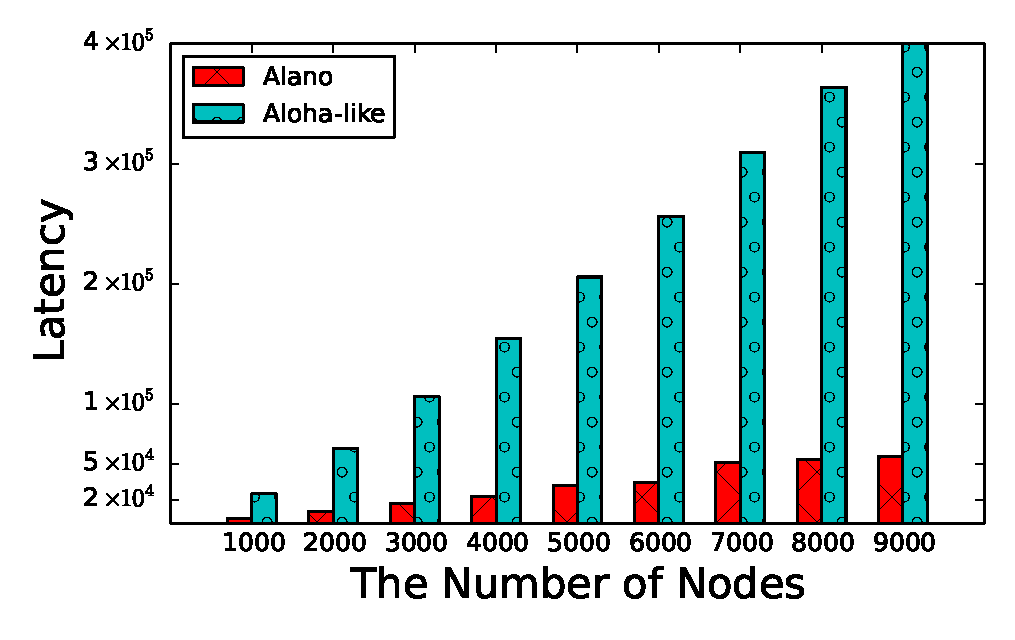
\includegraphics[width=1.65in]{Figure/node_uniform}}
\hspace{0.01in}
\subfigure[Normal Distribution]{\includegraphics[width=1.65in]{Figure/node_normal}}
\caption{Alano achieves lower latency with different number of nodes.}
\label{fig_node}
\end{figure}

\emph{Network Density} 




% This section will talk about conclusion of the paper
\section{Conclusion}
The conclusion goes here.

\bibliographystyle{IEEEtran}
\bibliography{ref}

\end{document}

\grid